A popular substream management method is the punctuation framework~\cite{tucker2003exploiting} applied in many production-scale SPEs such as Flink~\cite{carbone2015apache}, Heron~\cite{Kulkarni:2015:THS:2723372.2742788}, Samza~\cite{Noghabi:2017:SSS:3137765.3137770}, IBM Streams~\cite{jacques2016consistent}, Apex~\cite{pathak2016introduction}. The main idea behind this framework is to divide the stream by injecting special elements called {\em punctuations} that define substreams ``borders''. An SPE propagates these special elements via the same network channels as data elements. While the punctuation approach is robust and easy to implement, it has several limitations. 

Punctuations are not applicable for cyclic dataflows in a general case because elements belonging to a substream can remain in transit within a cycle for an uncertain time~\cite{carbone2018scalable}. Cyclic dataflows are commonly used for the distributed implementation of iterative web-graph algorithms like PageRank or search for connected components~\cite{ewen2012spinning, murray2016incremental, mcsherry2013differential}.

The technique proposed in~\cite{Carbone:2017:SMA:3137765.3137777} mitigates this issue for the state snapshotting problem. The main idea of this technique is to include in a snapshot all in-transit elements (possibly from previous epochs) within a cycle and then resend them on rollback. However, it does not allow a system to determine a substream termination for cyclic dataflows using punctuations.

As we demonstrated in the previous chapter, the high network overhead forms another limitation. Network traffic complexity for this method is $O(K|\Pi|^2)$, where $|\Pi|$ is the number of processes and $K$ is the number of substreams because each process should propagate punctuations to all output channels. The above formula estimates the number of punctuation messages needed in the worst case of fully interconnected processes. 

We argue that the worst case can appear on any execution graph that contains a re-partitioning operator. Indeed, SPEs try to distribute workload evenly between processes~\cite{carbone2015apache, Kulkarni:2015:THS:2723372.2742788, Akidau:2013:MFS:2536222.2536229}, so elements of a substream can be evenly distributed among processes as well. When a process reaches the end of a substream, it must broadcast the punctuation because the items of the part of a sub-stream handled by this process are re-distributed evenly for subsequent processing.

Substreams can be {\em fine-grained}: for example, each user session defines a substream. If there are a lot of small substreams, an inefficient substream management system can degrade the latency~\cite{DBLP:journals/pvldb/BegoliACHKKMS21} and the throughput of an SPE~\cite{Li:2008:OPN:1453856.1453890} or affect the performance of state checkpointing~\cite{zhang2021research}.

\begin{figure}[t]
  \centering
  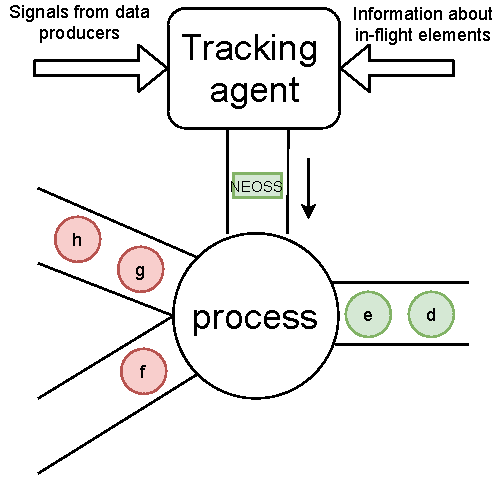
\includegraphics[width=0.60\textwidth]{Chapters/Tracker/pics/tracker-scheme.pdf}
  \caption{\tracker\ framework: tracking agent aggregates information about substreams and produces NEOSS}
  \label{tracker_scheme}
\end{figure}

In this chapter, we introduce a new substream management framework called \tracker. Figure~\ref{tracker_scheme} shows the high-level scheme of our method. 
Within this framework, we use a dedicated agent that receives information about substreams from the entire SPE and sends back {\em end-of-substream notifications} (NEOSS). 
An SPE propagates NEOSS messages through this agent without broadcasting between processes, reducing the amount of extra traffic. This propagation method is suitable for cyclic dataflows because there is no need to forward service traffic through the cycles. A distributed version of the agent allows an SPE to scale.

% In summary, our contributions are as follows:
% \begin{enumerate}
%     \item We provide a formal model of substream management. This model allows us to compare the properties of various substream management systems.
%     \item We present a novel substream management technique that achieves a lower bound of network traffic overhead.
%     \item We demonstrate \tracker\ performance compared to a state-of-the-art approach on diverse workloads.
% \end{enumerate}

% This paper is an extended version of a conference publication~\cite{10.1145/3524860.3539809}. This paper addresses a scalability problem by introducing a distributed version of the tracking agent and evaluating it on workloads with increased load. We further expand the theoretical properties of punctuation and tracker frameworks and reveal the motivation behind this work in more detail.

We organize the rest of the chapter as follows: 
% Section~\ref{fs-acker-preliminaries} formalizes the substream management problem and indicates its main properties. In Section~\ref{fs-acker-tracker}, we introduce a general design of the \tracker\ framework and demonstrate the properties of this substream management solution. Section~\ref{fs-acker-impl} summarizes the implementation of \tracker\ for both centralized and distributed setups with optimizations that can reduce the amount of extra traffic. In Section~\ref{fs-experiments}, we show that the proposed technique is scalable and can outperform alternatives employed in state-of-the-art stream processing engines. Section~\ref{fs-acker-related} outlines the relevant prior research. Finally, we discuss our conclusions in Section~\ref{fs-acker-conclusion}.